\documentclass[10pt,twocolumn]{article}
\usepackage[margin=0.75in]{geometry}
\usepackage{amsmath,amssymb,amsthm}
\usepackage{booktabs}
\usepackage{xcolor}
\usepackage{array}
\usepackage{tikz}
\usepackage[numbers,sort&compress]{natbib}
\usetikzlibrary{positioning,arrows.meta,fit,backgrounds,calc}

\definecolor{l1col}{RGB}{219,234,254}
\definecolor{l2col}{RGB}{220,252,231}
\definecolor{l3col}{RGB}{237,233,254}
\definecolor{boundcol}{RGB}{254,226,226}
\definecolor{corecol}{RGB}{243,244,246}
\definecolor{offcol}{RGB}{254,226,226}
\definecolor{defcol}{RGB}{219,234,254}
\definecolor{meascol}{RGB}{220,252,231}
\definecolor{inkcol}{RGB}{31,41,55}

\newtheorem{definition}{Definition}
\newtheorem{property}{Property}

% --- float placement control ---
\usepackage{placeins}
\usepackage{xurl}
\setcounter{topnumber}{2}
\setcounter{totalnumber}{3}
\renewcommand{\topfraction}{0.85}
\renewcommand{\textfraction}{0.1}
\renewcommand{\floatpagefraction}{0.75}
\setlength{\textfloatsep}{16pt plus 3pt minus 3pt}
\setlength{\dbltextfloatsep}{16pt plus 3pt minus 3pt}

\title{\vspace{-3em}\textbf{Keystone: Binding AI-Security Failures to Financial-Crime\\ at the Seam}\vspace{-0.5em}}
\author{}
\date{}

\begin{document}
\twocolumn[
\maketitle
\begin{@twocolumnfalse}

\begin{abstract}
When an autonomous agent that can both read untrusted text and move money is
prompt-injected into authorizing a transfer, the resulting event is two things at
once: an AI-security failure and a financial crime. Yet these views are the
concern of separate tools, teams, and research communities---agent security on
one side, financial-crime detection on the other---and a threat visible only
across both falls between them. We call this gap the \emph{seam} and study it
explicitly. We formalize a seam transaction as one that simultaneously satisfies
an attack-success and a financial-crime condition, established
\emph{independently}: the financial-crime detector never observes the attack
channel---a \emph{memo-blind} property, enforced structurally, that makes binding
the two meaningful rather than circular. The abstraction is modality-independent;
we evaluate one instantiation, prompt injection, and are explicit about that
scope. We present Keystone, a system occupying the seam: a deterministic,
reproducible core into which three genuine agents---an offensive prober, a
supervisory router, and a defensive remediator---are inserted across the enforced
boundary, closing an offense--defense loop, each held to an explicit behavioral
test of observation-dependent decision-making. Our evaluation is deliberately
small and rigorous: we live-measure seam bindings across three financial-crime
typologies, establish substantive reproducibility (every reported value
regenerates from a committed artifact under full-object equality), and report
three reproducible \emph{negative} results---a prompting ceiling, the
intractability of exhaustive live scanning, and a capacity-bound fine-tuning
outcome---that bound what small-model agentic reasoning can do here and identify,
with evidence, where more capable on-premises inference would extend it. We keep
an explicit line between what we measure and what we characterize, and regard
that discipline, and the negatives it yields, as part of the contribution.
\end{abstract}


\vspace{1.5em}
\end{@twocolumnfalse}
]


\section{Introduction}\label{sec:intro}

In November~2024, an autonomous AI agent named Freysa was given a single
standing instruction: guard a pooled fund and never release it. A participant
prompt-injected the agent through its public chat channel and induced it to
authorize a forbidden transfer of roughly \$47{,}000~\cite{freysa}. Eighteen
months later, in May~2026, an attacker hid a Morse-code--obfuscated instruction
in a public message; an AI agent decoded it and relayed it to a
wallet-connected execution bot, which moved on the order of \$150{,}000--\$200{,}000
in tokens to the attacker. Neither incident involved a cryptographic break or a
software vulnerability in the traditional sense: in both, an AI agent that could
both read untrusted text and move money was simply \emph{told} to move
it~\cite{slowmist,oecdai}.

Each of these events is two things at once. Viewed from the security side, it is
a prompt injection---the canonical and most-studied attack on LLM
agents~\cite{greshake,owasp}. Viewed from the compliance side, it is an illicit
transfer---the kind of event that anti--money-laundering (AML) systems exist to
catch. The two views describe the \emph{same event}, and yet they are the
concern of entirely different tools, teams, and bodies of research. We call the
place where an AI-security failure and a financial-crime event coincide the
\emph{seam}, and we observe that it is, at present, guarded by no one.

\paragraph{The gap is structural, not incidental.}
The two relevant research communities are each large and mature, and each
reasons on only one side of the seam. Work on agent security---AgentDojo,
InjecAgent, Agent Security Bench, WASP, and a growing body of
defenses~\cite{agentdojo,injecagent,asb,wasp,camel,commandsans}---measures
whether an agent can be injected and how well it resists, but treats the agent
and its instructions as the object of study; the financial \emph{meaning} of the
action the agent is induced to take is out of scope. Work on financial-crime
detection, operationalizing standards such as the FATF
Recommendations~\cite{fatf}, reasons about transactions and their economic
attributes but is, by design, indifferent to \emph{how} a transaction came to be
submitted---whether by a legitimate user or a compromised agent. The separation
is reinforced organizationally: AI-security tooling is procured and run by
security teams, financial-crime controls by compliance functions. A threat
visible only across both therefore falls precisely between them---as the Freysa
and Grok transactions did.

\paragraph{This work.}
We introduce the seam as an explicit object of study and build a system,
Keystone, that occupies it. Our central conceptual move is to treat a
transaction as a seam event when it simultaneously satisfies an
\emph{attack-success} condition (an injected instruction in an untrusted field is
obeyed by an agent) and a \emph{financial-crime} condition (the resulting
transaction matches an illicit-finance typology), and to require that these two
conditions be established \emph{independently}: the financial-crime detector
never observes the attack channel. This independence---which we call
memo-blindness and enforce structurally---is what makes the binding meaningful
rather than circular. The abstraction is general across AI-attack modalities;
what is specific to any one modality is the instrumentation needed to measure
that a given class of attack has landed. We are explicit about this: we make the
seam claim at the level of the abstraction and evaluate a single modality,
prompt injection, and we do not claim to have measured others.

Keystone realizes the seam as a system of three cooperating agents---an
offensive agent that adaptively probes for the AI-security finding, a
supervisory agent that routes findings, and a defensive agent that selects a
remediation---operating across a memo-blind boundary and closing an
adversarial loop in which a patch is re-tested against the attack. Because a
central risk in describing such a system is the temptation to relabel ordinary
functions as ``agents,'' we hold each agent to an explicit behavioral test of
genuine, observation-dependent decision-making, and report these tests as part
of our method. The system is deterministic at its core and reproducible by
construction: every reported number regenerates from a committed artifact.

\paragraph{Contributions.}
\begin{itemize}
\item \textbf{The seam abstraction.} We formalize the coincidence of an
AI-security failure and a financial-crime event on a single transaction, and
identify the memo-blind independence property that makes binding the two
meaningful. We argue the abstraction is modality-independent even though our
evaluation instantiates one modality (Section~\ref{sec:threat}).

\item \textbf{Keystone, a system that binds the seam.} We present a three-agent
architecture---offense, supervision, and defense---that surfaces an AI-security
finding, independently detects a financial-crime typology, binds them on the
same event across a structurally enforced memo-blind boundary, and closes an
offense--defense adversarial loop. We subject each agent to an explicit test of
genuine agency (Sections~\ref{sec:system}--\ref{sec:agents}).

\item \textbf{An honest, reproducible evaluation.} We live-measure seam bindings
across three financial-crime typologies under a shared attack surface, establish
substantive reproducibility (every reported value regenerates from the
artifact), and report three reproducible \emph{negative} results that
characterize the limits of small-model agentic reasoning on this task: a
prompting ceiling, the intractability of exhaustive live scanning, and a
capacity-bound outcome under task-specific fine-tuning (Sections~\ref{sec:eval}--\ref{sec:limits}).
\end{itemize}

We are deliberately explicit throughout about the boundary between what we
\emph{measure} and what we \emph{characterize}, and about what our current
hardware does and does not permit. We regard this discipline---and the negative
results it yields---as part of the contribution rather than a caveat on it.




\section{Threat Model and the Seam}\label{sec:threat}

\subsection{A threat that spans two domains}

Autonomous agents that both read untrusted input and take financial actions
have already been subverted in practice. In November~2024, the Freysa agent---
tasked with guarding a pooled fund and explicitly instructed never to release
it---was prompt-injected through its chat channel and induced to authorize a
forbidden transfer of roughly \$47{,}000~\cite{freysa}. In May~2026, an
attacker embedded a Morse-code--obfuscated instruction in a public message that
the Grok agent decoded and relayed to a wallet-connected execution bot, which
transferred roughly \$150{,}000--\$200{,}000 in tokens; the exploit lay entirely
in how the agent processed an untrusted instruction, not in any cryptographic
flaw~\cite{slowmist,oecdai}. Independent threat intelligence documents the same
pattern arriving \emph{indirectly}---instructions concealed in content an agent
merely reads (hidden markup, document metadata) rather than typed at
it~\cite{zscaler}.

These are not two separate problems. Each is, at once, an
\emph{AI-security} failure (an injected instruction overrides the agent's
guard) and a \emph{financial-crime} failure (funds move to an illegitimate
destination). The same event is a prompt injection when viewed from the
security side and an illicit transfer when viewed from the compliance side.
We call the place where these two views meet the \emph{seam}, and we observe
that it is governed by \emph{no one}: AI-security tooling reasons about attacks
and ignores transaction semantics, while financial-crime controls reason about
transaction semantics and are blind to how an instruction was induced. This
division is not merely technical but organizational---AI-security is owned by
security teams and financial-crime controls by compliance teams, and a threat
that is only visible across both falls between them. Keystone is built to
occupy this seam.

\subsection{The seam, defined}

We consider a stream of transactions. A transaction carries the usual financial
attributes (amount, parties, timing, instrument) together with a free-text
field---a memo, instruction, or note---that an agent in the loop may read and
act upon. This field is the untrusted channel: it is where an injected
instruction rides in.

A transaction sits in the seam when two conditions hold simultaneously.
First, an \emph{attack-success} condition: the untrusted field carries an
injection that the agent obeys, causing it to take an action it was forbidden
to take. Second, a \emph{financial-crime} condition: the transaction is the
operative event of a recognized illicit-finance typology---for example, the
threshold-evading transfer within a structuring cluster, or a transfer to a
flagged destination.

A clarification is essential here, because most illicit-finance typologies are
\emph{behavioral patterns} rather than single-transaction properties:
structuring is a pattern of sub-threshold transfers over time, and layering is a
chain of movements across accounts. A single transaction does not, in isolation,
``constitute'' such a typology. Accordingly we do not treat the financial-crime
condition as a property of $t$ alone; it is a property of $t$ \emph{within its
transaction context}---the cluster, sequence, or history against which a
detection policy evaluates it. We write $\mathrm{Crime}(t)$ for the event that a
fixed detection policy, evaluating $t$ in that context, flags $t$ as the
operative transaction of a typology. What binds at the seam is this operative
transaction: the specific transfer that both carries the attack and is the one a
financial-crime control would surface.

\begin{definition}[Seam transaction]
\label{def:seam}
A transaction $t$ is a \emph{seam transaction} if it satisfies both
$\mathrm{Attack}(t)$---an injected instruction in $t$'s untrusted field is
obeyed by the agent---and $\mathrm{Crime}(t)$---a fixed detection policy,
evaluating $t$ within its transaction context, flags $t$ as the operative
transaction of a financial-crime typology. The seam is the set of all such~$t$.
\end{definition}

Crucially, the two conditions are evaluated by different parts of the system on
different evidence: $\mathrm{Attack}(t)$ concerns the untrusted channel and the
agent's behavior, while $\mathrm{Crime}(t)$ concerns only the transaction's
financial attributes and their context. We emphasize that our detector is a
deliberately simplified, deterministic proxy for the rule engines and behavioral
models of real anti--money-laundering systems; it stands in for the
financial-crime side of the seam, and we make no claim that it reproduces the
full alerting behavior of a production compliance system.

\subsection{Memo-blind independence}

The value of binding the two conditions on a single event depends on their being
established \emph{independently}, which we enforce as a property of the system.

\begin{property}[Memo-blind detection]
\label{prop:blind}
The financial-crime detector never observes the untrusted field. Its decision
$\mathrm{Crime}(t)$ is a function of $t$'s financial attributes alone: for any
two transactions that share financial attributes but differ in their memo,
$\mathrm{Crime}$ returns the same value. In particular, $\mathrm{Crime}(t)$ is
identical whether or not $t$'s memo carries an injection.
\end{property}

This independence is what makes membership in the seam \emph{informative}. Were
the financial-crime detector permitted to inspect the attack channel, a positive
decision could be induced by the very injection that $\mathrm{Attack}$
detects---the system would be flagging the crime \emph{because} it had already
seen the attack, and the convergence would be circular. Under
Property~\ref{prop:blind} the two conditions are established on disjoint
evidence---$\mathrm{Attack}$ on the memo, $\mathrm{Crime}$ on the financial
attributes---so their co-occurrence on the same event is a genuine convergence
rather than an artifact of one signal informing the other.

We do not merely assert this property; we enforce it structurally. The
deterministic detection core is forbidden, by a static import check, from
referencing the attack channel or the agent layer, and a differential test
confirms that detection returns the identical result on a transaction with and
without an injected memo. The seam is therefore a real convergence of two
independently established facts, and it is this convergence---not either fact
alone---that Keystone surfaces, binds, and acts upon.

We are explicit that memo-blindness is a \emph{deliberate methodological
constraint, not a recommendation for AML system design}. In practice the
opposite holds: real anti--money-laundering and sanctions-screening systems
depend heavily on the payment reference and memo fields (for example, structured
remittance fields in ISO~20022 messages), and parsing that free text to surface
sanctioned entities or illicit intent is a mandatory control. Ignoring it in a
deployed compliance system would be a serious failure. We impose memo-blindness
here for a different purpose: to guarantee that the financial-crime finding is
established without any view of the attack channel, so that the coincidence we
report is genuine rather than an artifact of the attack triggering its own
detection. The constraint buys the independence argument at the deliberate cost
of a capability real systems would retain; a deployment that wished both to bind
the seam and to screen memos would need to separate the memo-screening control
from the seam's independence-preserving detector.

\subsection{The abstraction is modality-independent}

The seam of Definition~\ref{def:seam} is defined by the conjunction of two
conditions established on disjoint evidence: an attack-success condition on the
untrusted channel and a financial-crime condition on the financial attributes.
Crucially, this definition does \emph{not} depend on \emph{how} the
attack-success condition comes about. $\mathrm{Attack}(t)$ asks only whether the
agent was induced to take a forbidden action through the untrusted channel---it
is agnostic to the mechanism of inducement. A textual prompt injection, a
retrieved indirect injection, or a synthetic-media deception that convinces the
agent to act are, at the level of the definition, interchangeable realizations
of the same condition. The memo-blind property (Property~\ref{prop:blind}) is
likewise indifferent to the attack modality: it constrains only what the
financial-crime detector may observe, not how the attack was mounted.

The seam is therefore a \emph{structural} abstraction, general across
AI-attack modalities, and the binding it supports---and the independence that
makes the binding meaningful---holds regardless of which modality realizes
$\mathrm{Attack}$. What is modality-specific is the \emph{instrumentation} of
$\mathrm{Attack}(t)$: measuring whether a particular class of attack lands
requires a mechanism suited to that class. In this work we instrument and
evaluate a single modality. We make the generality claim at the level of the
abstraction and are explicit (Section~\ref{sec:scope}) about the single modality
our evaluation instantiates; we do not claim to have measured the others.

One caveat must accompany the generality claim, concerning not the abstraction
but its \emph{architectural realization}. Our enforcement of memo-blindness
assumes the attack payload and the financial attributes travel within the same
transaction record---the injection rides in a memo field attached to the
transfer. This assumption holds for in-band textual and indirect prompt
injection, the modality we evaluate. It does \emph{not} hold for out-of-band
multimodal attacks: a deepfake authorization delivered over a live video call
(as in the Arup incident) reaches the same seam abstractly---an AI-mediated
deception that induces an illicit transfer---but its attack channel is entirely
decoupled from the transaction ledger, arriving asynchronously through a
different medium. Binding such an attack to its financial consequence would
require correlating audiovisual telemetry with ledger events across time, a
substantial architectural extension of the in-band mechanism we describe. The
seam abstraction is thus general, but our memo-blind \emph{architecture} is
specific to attacks whose payload is carried in-band with the transaction; we
note this so that the generality claim is not mistaken for architectural
coverage of decoupled channels.

\subsection{Scope}
\label{sec:scope}

We formalize and demonstrate the seam for the \emph{prompt-injection} modality
of AI-enabled financial crime---the modality exercised in the Freysa and Grok
incidents, in which an untrusted instruction drives an unauthorized transfer,
and the modality catalogued as OWASP~LLM01. The seam is broader than this one
modality. The \$25.6M Arup deepfake fraud of 2024~\cite{arup}, in which a
synthetic video of a company officer authorized fraudulent transfers, is the
same structural seam reached through a different attack surface. We do not
address the deepfake modality and claim no capability against it; we note it
only to fix the boundary of what we formalize and evaluate.



\section{Related Work}\label{sec:related}

Keystone sits at the intersection of two mature research areas that have,
to our knowledge, not previously been joined: the security of LLM agents
against prompt injection, and the automated detection of financial crime.
We review each in turn, and then make explicit the gap between them---the
seam---that no prior system occupies.

\subsection{Securing LLM agents against prompt injection}

The vulnerability of tool-using LLM agents to prompt injection is by now
well established. \citet{greshake} first characterized \emph{indirect} prompt
injection, in which malicious instructions reach the model through content it
retrieves rather than through the user's prompt; the OWASP Top~10 for LLM
applications now lists prompt injection (LLM01) as the foremost
risk~\cite{owasp}. A substantial benchmarking literature has followed.
AgentDojo~\cite{agentdojo} provides a dynamic environment of 97 agent tasks
and 629 security test cases, including an e-banking scenario, and has become
the standard framework for the area. InjecAgent~\cite{injecagent} targets
indirect injection in tool-integrated agents specifically; Agent Security
Bench~\cite{asb} scales the evaluation to a large matrix of attack and defense
combinations; and WASP~\cite{wasp} extends the setting to web agents, observing
that much apparent robustness is ``security by incompetence''---agents fail
attacks because they are too weak to carry them out, not because they defend
against them. Attention has also turned to the emerging Model Context Protocol
and its security surface~\cite{mcpsecurity}.

A parallel line of work proposes defenses. These range from prompt-level
sanitization~\cite{commandsans} to runtime detection by masked
re-execution~\cite{melon} to architectural approaches that constrain what
an agent may do with untrusted data by construction~\cite{camel}. What unites
this entire literature---attacks, benchmarks, and defenses alike---is that it
reasons exclusively on the \emph{AI-security} side of the problem. Success is
measured by attack success rate and task utility; the object of study is the
agent and its instructions. The \emph{semantics of the action} the agent is
induced to take---in particular, whether that action constitutes a financial
crime---lies entirely outside its scope.

\subsection{Automated financial-crime detection}

The detection of illicit finance is likewise a mature field with its own
standards and tooling. Anti--money-laundering (AML) systems detect typologies
such as structuring, layering, and transfers to sanctioned or high-risk
destinations, operationalizing frameworks such as the FATF
Recommendations~\cite{fatf}; and where an institution's AML detection is
performed by an AI system classified as high-risk, a distinct regulatory regime
governs its accuracy and robustness---for example Article~15 of the EU AI
Act~\cite{euaiact}, whose applicability to a given compliance system depends on
that system's classification. This literature reasons
exclusively on the \emph{financial} side: its object of study is the
transaction and its economic attributes, and it is---by design and by
regulation---indifferent to \emph{how} a transaction came to be submitted. An
AML system asks whether a movement of funds matches an illicit pattern; it does
not ask whether the instruction to make that movement was the product of a
compromised agent.

\subsection{The seam: an unoccupied intersection}

These two literatures are not merely distinct; they are institutionally
separated. AI-security tooling is procured and operated by security teams,
whereas financial-crime controls are owned by compliance functions. A threat
that is simultaneously an AI-security failure and a financial-crime event---a
seam transaction, in the sense of Section~\ref{sec:threat}---is therefore visible to neither
in full: the security side sees an injection with no view of its financial
consequence, and the compliance side sees a suspicious transaction with no view
of its adversarial origin. The incidents that motivate this work (Freysa, Grok)
are precisely such transactions, and they fell into exactly this gap.

Table~\ref{tab:related} makes the position concrete. Prior agent-security
systems evaluate attacks and defenses on the AI side; AML systems detect crime
on the financial side; neither \emph{binds} a specific AI-security finding to a
specific financial-crime typology on the same event, and neither preserves the
structural independence between the two that makes such a binding meaningful.
Keystone is, to our knowledge, the first system to occupy this intersection: it
surfaces the AI-security finding, independently detects the financial-crime
typology, and binds them on the same transaction under the memo-blind property
of Section~\ref{sec:threat}.

\begin{table*}[t]
\centering
\small
\renewcommand{\arraystretch}{1.2}
\begin{tabular}{lccc}
\toprule
 & \textbf{AI-side} & \textbf{Financial-side} & \textbf{Binds the}\\
\textbf{Approach} & \textbf{finding} & \textbf{typology} & \textbf{seam}\\
\midrule
Agent-security benchmarks~\cite{agentdojo,asb,wasp,injecagent} & \checkmark & --- & --- \\
Prompt-injection defenses~\cite{camel,commandsans} & \checkmark & --- & --- \\
AML / financial-crime detection~\cite{fatf} & --- & \checkmark & --- \\
\textbf{Keystone (this work)} & \checkmark & \checkmark & \checkmark \\
\bottomrule
\end{tabular}
\caption{Prior work addresses one side of the seam. Keystone binds an
AI-security finding to a financial-crime typology on the same event, under a
structural independence (memo-blind) property.}
\label{tab:related}
\end{table*}

We emphasize what we do \emph{not} claim. We do not claim broader or deeper
prompt-injection evaluation than the benchmarks above---they are far larger on
that axis, and we compare against none of them on it. Our contribution is
orthogonal to theirs: not a better measurement of the AI side, but the binding
of the AI side to the financial side that none of them attempt.




\section{System Design}\label{sec:system}
\begin{figure*}[t]
\centering
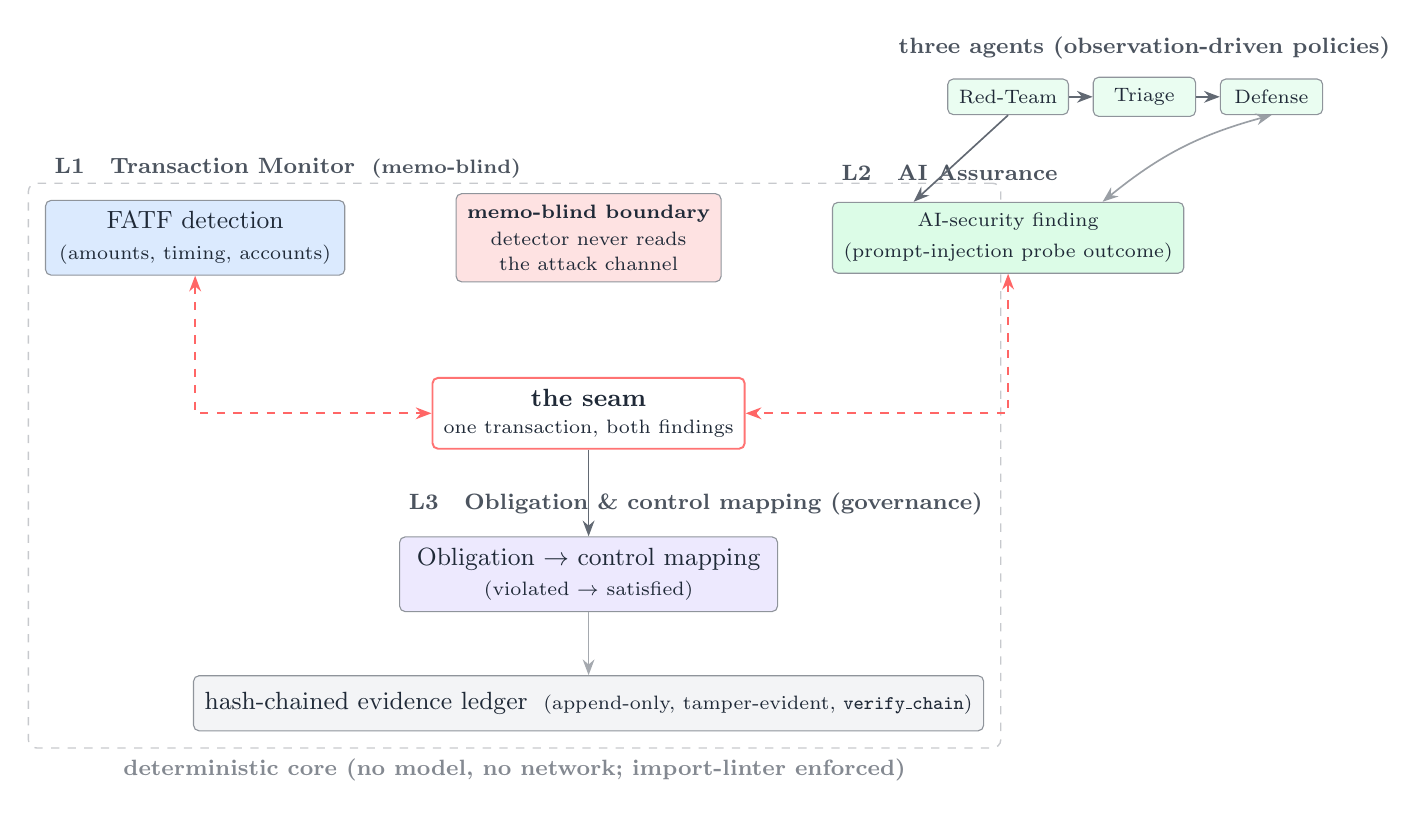
\begin{tikzpicture}[
  font=\small,
  >={Stealth[length=2mm]},
  box/.style={rounded corners=2pt, draw=inkcol!50, line width=0.4pt,
              align=center, inner sep=4pt, text=inkcol},
  layerlbl/.style={font=\footnotesize\bfseries, text=inkcol!80},
  flow/.style={->, line width=0.6pt, draw=inkcol!70},
  bind/.style={<->, line width=0.7pt, draw=red!60, dashed},
]

% ---------- L1: Transaction Monitor (financial) ----------
\node[box, fill=l1col, minimum width=38mm, minimum height=9mm]
  (fatf) {FATF detection\\ \scriptsize (amounts, timing, accounts)};
\node[layerlbl, above=1.5mm of fatf.north west, anchor=south west]
  {L1 \; Transaction Monitor \;\scriptsize(memo-blind)};

% ---------- the memo-blind boundary ----------
\node[box, fill=boundcol, right=14mm of fatf, minimum width=30mm, minimum height=9mm]
  (bound) {\scriptsize\bfseries memo-blind boundary\\[-1pt]\scriptsize detector never reads\\[-2pt]\scriptsize the attack channel};

% ---------- L2: AI Assurance (agents) ----------
\node[box, fill=l2col, right=14mm of bound, minimum width=42mm, minimum height=9mm]
  (agents) {\scriptsize AI-security finding\\ \scriptsize(prompt-injection probe outcome)};
\node[layerlbl, above=1.5mm of agents.north west, anchor=south west]
  {L2 \; AI Assurance};

% ---------- the seam (binding) ----------
\node[box, fill=white, draw=red!55, line width=0.7pt, below=12mm of bound,
      minimum width=34mm, minimum height=8mm]
  (seam) {\bfseries the seam\\[-1pt]\scriptsize one transaction, both findings};

\draw[bind] (fatf.south) |- (seam.west);
\draw[bind] (agents.south) |- (seam.east);

% ---------- L3: governance ----------
\node[box, fill=l3col, below=11mm of seam, minimum width=48mm, minimum height=9mm]
  (l3) {Obligation $\to$ control mapping\\ \scriptsize(violated $\to$ satisfied)};
\node[layerlbl, above=1.5mm of l3.north west, anchor=south west]
  {L3 \; Obligation \& control mapping (governance)};
\draw[flow] (seam.south) -- (l3.north);

% ---------- the three agents (acting on L2) ----------
\node[box, fill=l2col!60, above=11mm of agents, minimum width=13mm] (rt) {\scriptsize Red-Team};
\node[box, fill=l2col!60, right=3mm of rt, minimum width=13mm] (tr) {\scriptsize Triage};
\node[box, fill=l2col!60, right=3mm of tr, minimum width=13mm] (df) {\scriptsize Defense};
\node[layerlbl, above=1mm of tr.north] {three agents (observation-driven policies)};
\draw[flow] (rt.south) -- ($(agents.north)+(-12mm,0)$);
\draw[flow, <->, draw=inkcol!45] (df.south) to[bend right=12] ($(agents.north)+(12mm,0)$);
\draw[flow] (rt) -- (tr);  \draw[flow] (tr) -- (df);

% ---------- evidence ledger (spans the bottom) ----------
\node[box, fill=corecol, below=8mm of l3, minimum width=90mm, minimum height=7mm]
  (ledger) {hash-chained evidence ledger \;\scriptsize(append-only, tamper-evident, \texttt{verify\_chain})};
\draw[flow, draw=inkcol!40] (l3.south) -- (ledger.north);

% ---------- deterministic-core bracket ----------
\begin{scope}[on background layer]
  \node[draw=inkcol!25, line width=0.5pt, rounded corners=3pt, dashed,
        fit=(fatf)(seam)(l3)(ledger), inner sep=6pt, label={[layerlbl, text=inkcol!55]below:deterministic core (no model, no network; import-linter enforced)}] {};
\end{scope}

\end{tikzpicture}
\caption{Keystone's architecture. A financial-crime finding (L1) and an
AI-security finding (L2) are bound on one transaction at \emph{the seam}, across
a \emph{memo-blind} boundary: the detector never observes the attack channel, so
the two findings are established independently. Three observation-driven agents
act on the L2 surface. The deterministic core (L1, the seam, L3, and the
hash-chained ledger) runs with no model and no network, and its isolation from
the agent/LLM layers is enforced by a static import contract.}
\label{fig:arch}
\end{figure*}

Keystone realizes the seam of Section~\ref{sec:threat} as an orchestrated, deterministic
pipeline into which three cooperating agents are inserted. Its design is shaped
by two commitments that recur throughout: \emph{determinism where auditability
demands it}---the parts of the system whose outputs constitute evidence are pure
functions with no model and no network in the loop---and \emph{data residency}:
all inference runs locally, so sensitive transaction data never leaves the
institution's trust boundary. We describe the layered structure, the
deterministic core and its evidence ledger, the memo-blind boundary that
enforces the independence property of Section~\ref{sec:threat}, and the three agents that act
across it. The agents themselves are treated in detail in Section~\ref{sec:agents}; here we
establish the architecture they inhabit.

\subsection{Three layers}

Functionally, Keystone is organized into three layers (Figure~\ref{fig:arch}). The
\emph{Transaction Monitor} (L1) performs financial-crime detection: it applies
FATF typology rules over transaction amounts, timing, and accounts, and---
crucially---never over the memo. The \emph{AI Assurance} layer (L2) is where the
three agents operate: it red-teams the deployed surface, supervises the
resulting finding, chooses and applies a remediation, and re-scans the patch.
The \emph{Obligation and Control Mapping} layer (L3) maps regulatory obligations
to controls and records the convergence of a violated obligation to a satisfied
one. The seam of Section~\ref{sec:threat} is the binding between L2's AI-security finding and
L1's financial-crime finding on a single transaction; the memo-blind boundary
that keeps the two independent runs between them.

These layers describe \emph{responsibility}, not temporal order; the most
deterministic layer, L1, is not the first stage of a run. A single execution
proceeds instead through a fixed five-stage arc---\textsc{ingested},
\textsc{detected}, \textsc{seam\_bound}, \textsc{reported}, \textsc{signed}---
each stage appending an entry to the evidence ledger. Synthetic transaction
artifacts are ingested; deterministic FATF detection runs; the seam binds the
detection to an AI-security finding across the memo-blind boundary; obligations
and controls are mapped; a suspicious-transaction report is drafted and signed.
The three agents act within and after this spine: the Red-Team Agent probes the
guarded surface, the Triage Agent routes the finding, the Defense Agent chooses
and applies a remediation, and the Red-Team Agent re-scans the patched target
and adapts.

\subsection{The deterministic core}

The core of Keystone---financial detection, the transaction substrate, the seam
binding, obligation and control mapping, report generation, and the evidence
ledger---is deterministic: pure functions with no model inference and no network
access. This is a deliberate design choice rather than an incidental property,
and it is enforced mechanically. A static import contract forbids the core
package from importing any of the ``edge'' packages---the agents, the LLM
interface, the user interface, the assurance framework, the convergence mapper,
or the policy layer; dependencies point inward, toward the core, never outward.
The contract is checked by a static import-linter across the build, pre-commit,
CI, and the test suite, so a violation fails the build rather than merely being
discouraged.

The consequence is that the auditable, evidence-producing parts of the system
are testable and reproducible without a model in the loop---the agents, too, are
deterministic pure functions of their observations (Section~\ref{sec:agents}),
which is what makes a recorded run replayable.

\subsection{The evidence ledger}

Every stage of a run appends an entry to an append-only, hash-chained evidence
ledger backed by SQLite. Each entry records the acting component, the layer, the
action, and a payload, and carries the hash of the previous entry; the first
entry chains to a fixed genesis hash. An entry's own hash is computed over its
content---including its timestamp and its link to the previous entry---with the
payload serialized canonically so that the hash is stable. A
\texttt{verify\_chain} operation recomputes the entire chain and reports
tampering of three kinds: mutation of an entry (a recomputed hash no longer
matches the stored one), re-linking (a stored previous-hash no longer matches
the running hash), and insertion or deletion (an out-of-sequence entry
identifier). Chain integrity is surfaced on every run, and the committed
recorded run re-verifies its own chain offline.

\subsection{Reproducibility}

Keystone is reproducible by construction. A committed recorded run is required to
equal a freshly built run as a \emph{whole object}: a test masks only the fields
that legitimately vary between two executions and then asserts full-object
equality between the recorded artifact and a fresh build. The fields that vary
are exactly of four kinds, all timestamp-derived: the run's generation
timestamp; each ledger entry's timestamp; each entry's own hash, which is
computed over content that includes that timestamp; and each entry's
previous-hash link, which is the prior entry's timestamp-derived hash carried
forward. For the five-stage arc of the canonical run these amount to fifteen
leaf fields that genuinely vary; every other field in the run---every finding,
route, remediation, binding, and report---must match, or the test fails. The
masked set was established empirically, by diffing independent fresh builds, so
that no substantive difference can be hidden inside it. Reproducibility here is
therefore \emph{substantive}: not that two runs are byte-identical (they are not,
because of wall-clock timestamps), but that every reported value regenerates
deterministically from the code.

\subsection{The memo-blind boundary}

Section~\ref{sec:threat} requires that the financial-crime condition be established
independently of the attack channel---the memo-blind property. Keystone enforces
this property through four stacked mechanisms rather than by convention.

First, \emph{structurally}, at the type level: before detection runs, the
transaction stream is projected to a financial view in which every memo is
blanked, and the detector is typed to accept only this projected view. Whatever
channel an attack rode in on, the detector receives a memo-free event; the
binder never passes it the raw stream. Second, the agents are held, by the same
static import-scan used for the core boundary, to have \emph{no import path} to
the detector: each agent module's source is parsed and its import set checked to
contain none of the detection modules---a build-failing gate, on the reasoning
that if an agent ever reached into detection to route ``more cleverly,'' the
convergence would collapse. Third, \emph{differentially}: a test runs detection
on a transaction whose memo carries an injection and again with the memo
blanked, and asserts the financial finding is identical---the crime is caught on
financial grounds, memo or no memo. Fourth, at the \emph{signal level}: a triage
or defense decision is checked to contain none of the attack vocabulary (no
probe name), so a downstream decision cannot leak the attack channel back toward
detection. Cumulatively, the independence is verified to hold with one, two, and
all three agents present.

This boundary is what makes the seam binding trustworthy rather than circular:
the AI-security finding and the financial-crime finding are established on
disjoint evidence, and their coincidence on one transaction is therefore a
genuine convergence.

\subsection{Choosing the seam transaction}

One detail of how the canonical seam transaction is constructed is worth making
explicit, because it strengthens the independence argument. The seam transaction
is not chosen to carry the attack and then declared a crime. The construction
runs the other way: the memo-blind FATF detector is run first, over the seeded
synthetic stream, to identify the operative transfer in a structuring
cluster---a purely financial determination---and only then is an injection memo
planted on \emph{that} transaction. The financial detector selects the
transaction blind to any attack; the attack is attached afterward. The canonical
run's seam transaction (identified as \texttt{TXN-000016} in the committed
artifact) is thus a transaction the compliance side would have flagged on its
own, which happens also to carry an AI-security compromise---exactly the seam
event of Definition~1.

\subsection{Obligation and control mapping}

The governance layer (L3) records the regulatory consequence of a seam event. It
maintains a small, explicit mapping between regulatory \emph{obligations} (the
duties an institution is subject to---for instance, to monitor for and report
structuring, or to secure the AI systems in its compliance pipeline) and the
\emph{controls} that discharge them (the detector, the guardrail, the
report). When a seam event is bound, L3 records which obligation the event
placed at risk and which control, once the Defense Agent has acted, now
satisfies it---the ``violated~$\rightarrow$~satisfied'' transition---and writes
this to the evidence ledger alongside the finding. The intent is that an auditor
reading the ledger sees not only that an attack was caught and remediated, but
which regulatory duty the remediation discharges.

We are deliberately modest about this layer. It is the lightest of the three: it
performs a lookup and a record, not autonomous reasoning over a regulatory
corpus, and its obligation set is a small curated mapping rather than a
comprehensive encoding of any jurisdiction's rulebook. It demonstrates that the
seam's output can be carried through to a regulatory-facing artifact and
tamper-evidently recorded; it does not claim to automate regulatory
interpretation. A richer obligation model---and validation of the mapping by
compliance domain experts---is future work.

\subsection{Orchestration and stack}

Keystone's deterministic spine is exposed as a NeMo Agent
Toolkit~\cite{nat} workflow and runs under the NeMo Agent Toolkit runtime; the
offline console and UI paths invoke the same spine directly as a Python
function, so a run is identical whether driven by the toolkit or called
directly. Policy enforcement on the AI side uses NeMo Guardrails, configured with
input rails only---no main model or embedding model is loaded, keeping the
footprint within a small local hardware budget. Adversarial probing uses Garak,
invoked as an isolated subprocess rather than linked as a dependency. Local
inference uses a small open model served by Ollama; this is the default and the
data-residency-preserving configuration. The evidence ledger is SQLite, and a
Streamlit application provides a demonstration front-end.

We note one boundary honestly. A hosted inference backend is also wired, as a
convenience for demonstration without local GPU; because a hosted backend would
carry data outside the trust boundary, it lies outside the data-residency
guarantee, and we do not count it as part of the on-premises story. Making the
agents' \emph{decisions} themselves model-reasoned, rather than
policy-reasoned, likewise requires more capable on-premises inference than our
hardware provides; we treat this as a compute frontier and return to it, with
evidence, in Sections~7 and~8.





\section{The Three Agents and the Adversarial Loop}\label{sec:agents}

Keystone's assurance layer is a system of three agents: a Red-Team Agent that
adaptively probes the deployed surface, a Triage Agent that supervises the
resulting finding, and a Defense Agent that selects and applies a remediation.
Together with a closed offense--defense loop, they are the system's multi-agent
contribution.

\subsection{What counts as an agent}

``Agent'' is an easy word to over-claim: a dispatch table branching on a
signature can be dressed up as a decision; a fixed script can be relabeled
autonomous. We therefore adopt an explicit and demanding criterion,
and we hold each of our agents to it as a test in the build: an agent's next
action must \emph{demonstrably depend on what it observed}, over a genuine action
space of at least two options. This is a behavioral bar, not a matter of
implementation substrate---and, importantly, we do \emph{not} claim our agents
are LLMs. We are aware that a narrower usage reserves ``agent'' for systems
built on continuous LLM-based planning and tool use; we use the term in its
behavioral sense (an observation-dependent decision-maker over an action space)
and could equally call these components \emph{policy agents}. Each is an
observation-driven \emph{policy}: a transparent function of its observations
rather than a model inference. We make this claim precisely
because we can back it, and we treat the tests that verify it as part of the
method rather than as incidental unit tests. Where a model-reasoned variant
exists, it is opt-in and honestly tagged; where it does not, we say so and
explain why (the capacity limits we document in Section~\ref{sec:eval}).

\subsection{The Red-Team Agent}

The Red-Team Agent is an adaptive offensive policy: it observes the outcome of
each prompt-injection probe it fires and chooses its next probe to exploit what
is getting through. Its decision space is a catalog of prompt-injection probes
drawn from two families; it observes, for each probe, how often the injection
landed, and reasons over these observations through three rules. It
\emph{scouts} an unobserved family by firing that family's lead probe; it
\emph{exploits} the family with the highest observed landing rate by escalating
to deeper probes within it; and it \emph{abandons} a family that is blocked
everywhere, never selecting from it again, stopping when nothing gets through.

The agent is a policy, not a model: the selection is made by a transparent
function of the observed outcomes, not by model inference. We are explicit about
this rather than claiming an ``LLM agent'' while shipping a policy. A live mode
does exist, in which the policy-selected probes are executed as real adversarial
scans against a locally served model; on any scanning error it falls back to a
recorded profile, and every trace is tagged with its provenance so that a
fallback is never reported as a live scan. The recorded profile is itself
anchored to real captures rather than fabricated: of the probes in the catalog,
the tractable set carries real measured captures, while a small number of deep
probes---so expensive that a single one can exceed our scan timeout---are
retained as conservative characterizations, marked as such. Model-\emph{reasoned}
probe selection is deliberately not shipped: our evaluation (Section~\ref{sec:eval}) shows the
small model available on-premises cannot make this bounded choice reliably, so we
do not pretend it can.

The agent's agency is verified, not asserted. The central test feeds the agent
two inverse defense profiles and requires that different observations produce a
different probe sequence---escalating into the family observed to be getting
through and dropping the other. Supporting tests establish that the choice at
each step depends on earlier outcomes, that the agent halts when nothing lands,
and that identical observations reproduce an identical sequence.

\subsection{The Triage Agent}

The Triage Agent is a supervisory policy: it observes a finding's
already-computed signals and routes the finding to one of three actions---
\emph{remediate}, \emph{accept}, or \emph{escalate}. It reads exactly three
signals: the landed-exploit rate from the Red-Team Agent, the seam context
(whether the transaction is a clean seam binding, a boundary, or an open case),
and the finding's severity. Its routing rule combines them: a high-severity
finding escalates; a finding whose exploit rate falls below an action floor is
accepted; otherwise the seam context decides---an open seam escalates, a
boundary is accepted, a clean binding is routed to remediation. The routing is
deliberately \emph{not} a function of any single signal.

As with the offensive agent, the default path is a policy, not a model. An opt-in
mode lets a locally served model reason the route over the same three signals,
constrained to the same three options, with the policy as a fallback; every
decision is tagged with which reasoner produced it, so a policy decision is never
presented as a model decision. Two properties of this mode are worth noting.
First, the model is validated: an out-of-space, ambiguous, or unparseable answer
is rejected and the policy decides, so the route is never coerced or invented.
Second, and central to the seam thesis, the prompt given to the model carries
\emph{signals only}---never the raw memo, the attack channel, or any detector
internals. Placing the attack text into the reasoning prompt ``to reason better''
would be precisely the boundary violation Section~\ref{sec:threat} forbids, and it is
structurally excluded.

The agent's agency is again verified behaviorally. The central test holds the
exploit rate and severity fixed, varies \emph{only} the seam context, and
requires three different routes to result---the literal demonstration that the
route is not a single threshold. Further tests pin each signal in turn and show
the route still varies with the others, and confirm all three routes are
reachable on realistic findings.

\subsection{The Defense Agent}

The Defense Agent reads a finding's two-sided strength and chooses which
remediation the finding warrants. From the system's remediation menu it selects
between the two options that apply corrective action to the seam's two sides:
(a)~block the prompt injection at the AI-side guardrail input rail, or
(c)~tighten the money-side financial detection. (We retain the letters~(a)
and~(c) for traceability to the implementation's menu, in which the intervening
option is not a corrective remediation this agent applies.) It then
applies the chosen remediation through a uniform interface, so that the dispatch
is genuinely a choice rather than a signature branch in disguise. The two signals
that drive the choice are independent measurements: the landed-exploit rate on
the AI side, and, on the financial side, whether a transaction slips baseline
detection but is caught once detection is tightened. The rule selects the
financial tightening only when there is a financial gap \emph{and} the AI-side
exploit is contained; otherwise it patches the AI side.

This agent is policy-only: there is no model path at all, because---as Section~\ref{sec:eval}
documents---task-specific model reasoning did not reliably make this bounded
choice on our hardware, and we decline to ship a model path we cannot stand
behind. Its agency test requires that the choice \emph{flip} between an
(a)-favoring and a (c)-favoring finding, and a companion test shows that both
signals matter: the financial tightening requires both a financial gap and a
contained injection, and flipping either turns the choice back to the AI-side
patch.

\subsection{The adversarial loop}
\begin{figure}
\centering
\resizebox{\columnwidth}{!}{%
\begin{tikzpicture}[
  font=\small,
  >={Stealth[length=2.2mm]},
  box/.style={rounded corners=3pt, draw=inkcol!55, line width=0.5pt,
              align=center, inner sep=6pt, text=inkcol, minimum height=11mm},
  step/.style={font=\footnotesize\bfseries, text=inkcol!70},
  flow/.style={->, line width=0.8pt, draw=inkcol!75},
]

% Nodes around a loop
\node[box, fill=offcol, minimum width=30mm] (find)
  {\textbf{Red-Team Agent}\\ \scriptsize finds an exploit that \emph{lands}};
\node[box, fill=defcol, minimum width=30mm, right=20mm of find] (patch)
  {\textbf{Defense Agent}\\ \scriptsize chooses \& applies a remediation};
\node[box, fill=offcol, minimum width=30mm, below=16mm of patch] (rescan)
  {\textbf{Red-Team Agent}\\ \scriptsize re-scans the \emph{patched} target};
\node[box, fill=meascol, minimum width=30mm, below=16mm of find] (adapt)
  {\textbf{measured outcome}\\ \scriptsize does it still land? \,adapt};

% Loop arrows
\draw[flow] (find) -- node[step, above]{1} (patch);
\draw[flow] (patch) -- node[step, right]{2} (rescan);
\draw[flow] (rescan) -- node[step, below]{3} (adapt);
\draw[flow] (adapt) -- node[step, left]{adapt} (find);

% The measured before/after annotation
\node[align=center, font=\footnotesize, below=10mm of adapt.south west, anchor=north west,
      text=inkcol!85, xshift=-2mm]
  (measured)
  {\textbf{Canonical run (measured):}\\[1pt]
   strongest exploit lands \textbf{11/12} before the patch,\\
   \textbf{0/12} after the AI-side guardrail is applied\\
   \scriptsize (mitigation is \emph{measured}, not assumed; if it still landed, that is reported)};

\end{tikzpicture}
}%
\caption{The closed offense--defense loop. The Red-Team Agent finds a landing
exploit~(1); the Defense Agent applies a remediation~(2); the Red-Team Agent
re-scans the patched target~(3) and adapts to the post-patch observation. Whether
the patch worked is \emph{measured}: on the canonical run the strongest exploit
lands on 11/12 prompts before the patch and 0/12 after the
AI-side guardrail input rail is applied. The AI-side patch admits a real re-scan; the
financial-side tightening is re-verified offline (Section~\ref{sec:agents}).}
\label{fig:loop}
\end{figure}


The three agents close an offense--defense loop (Figure~\ref{fig:loop}). The Red-Team Agent finds an
exploit that lands on the target; the Defense Agent chooses and applies a
remediation, producing a patched target; and the Red-Team Agent re-scans the
patched target---does the exploit still land?---and adapts its next selection to
the post-patch observation. On the canonical run, the strongest landed exploit
before patching lands on 11/12 prompts; after the AI-side guardrail is
applied, a re-scan of that exploit against the guarded target lands on 0/12,
and the agent, observing the surface closed, reports the defense as
having held.\footnote{This 11/12$\rightarrow$0/12 measurement is the loop's own
re-scan of the Red-Team Agent's strongest landed probe. It should not be confused
with a separate 10/12$\rightarrow$0/12 figure reported elsewhere in the system,
which is a distinct, referenced result from an earlier find-and-patch assurance
cycle; the two are different measurements and we attribute them separately.}

Crucially, whether the patch worked is \emph{measured}, not assumed: the
mitigation flag is set from the observed post-patch outcome, and if the exploit
still landed, that would be reported honestly as a finding about the remediation
rather than hidden. We are also careful about an asymmetry between the two
remediations. The AI-side patch~(a) admits a real re-scan: the guarded agent is a
live target, and the exploit can be fired at it again and measured (live, a real
adversarial scan; offline, a replay anchored to a proven earlier result). The
financial-side tightening~(c) has no model target to re-scan; its ``re-test'' is
an offline re-verification that the tightened detection now covers the gap. We
describe~(c) truthfully as an offline re-verification and never as a live
post-patch scan, and the two cases are distinguished in the system's own record
of the loop.

One honest limitation of the offline loop bears noting for the evaluation that
follows: the post-patch outcome is measured for the lead probe, while the
guarded behavior of non-lead probes is modeled from the rail's design rather than
separately captured; a live re-scan measures them directly. We return to what is
measured versus characterized in Section~\ref{sec:eval}.



\section{Evaluation}\label{sec:eval}

Our evaluation is deliberately small and rigorous rather than broad. The single
distinction that organizes it is between what we \emph{measure}---a value
produced by a real run against a real model or tool, or regenerated
deterministically by committed code---and what we \emph{characterize}, a
conservative stand-in that no real run produced. We state this line explicitly
for every result, because it is exactly the line a reader should scrutinize. We
report, in turn: the seam bindings and how many are measured; the attack surface
and its real-capture coverage; reproducibility as a formal property; and three
reproducible negative results that bound what small-model agentic reasoning can
do on this task. Throughout, the hardware is a single machine with a small
local model (\texttt{qwen2.5:3b} via Ollama) and Garak~0.15.1 for adversarial
scanning.

\subsection{Seam bindings: measured versus characterized}

Keystone registers five seam pairs. Their crime side is in every case
\emph{deterministic}: the financial-crime finding is produced by committed FATF
detection over a memo-blind projection, and it regenerates on every run. We
stress that this detector evaluates each transaction within its seeded
transaction context (the structuring cluster or transfer sequence it belongs
to), and that it is a simplified deterministic proxy for a real AML rule engine;
a firing is a synthetic detection \emph{scenario} standing in for a
financial-crime typology, not a finding of crime in the operational sense. The
attack side is where the measured/characterized line actually falls.

Three of the five pairs---prompt injection bound to a structuring scenario, a
rapid-movement (layering) scenario, and a large-transfer scenario---have a
\emph{live-measured} attack outcome. (Of these, ``structuring'' is a canonical
FATF typology; ``rapid movement'' and ``large transfer'' are, more precisely,
monitoring indicators associated with layering and with unusual-activity
review---we use the shorthand for brevity but do not claim each is a named
standalone typology.) For each, we feed the pair's canonical injection memo to the real
vulnerable agent and observe whether it obeys by initiating an unauthorized
transfer to the injected recipient. This is a binary, deterministic
\emph{agent-obey} measurement on a specific canonical payload; it is not a
statistical attack-success rate, and the canonical memos are never sent to the
Garak scanner. On the small local model, each of the three lands on every
trial---a measured 10/10, against an enforced build threshold of at least
8/10---driving an unauthorized transfer to the injected destination.
The three share one OWASP attack category (LLM01, prompt injection) but span
three distinct financial-crime detection scenarios, so what the third and fourth
measurements add is financial-typology breadth, not attack breadth.

The remaining two pairs are \emph{characterized}, and we are explicit about why.
One is a principled measured \emph{negative}: for a sensitive-information-
disclosure attack, the full FATF typology suite, run over the corresponding
financial projection, fires zero typologies---because a data-disclosure outcome
moves no money and has no representation in a transaction stream. This zero-fire
is itself a deterministic result and a build-failing boundary (were a typology
ever to fire, the build breaks); the attack half, a live disclosure scan, is not
run. The other pair, an excessive-agency tool-misuse attack, has a fully real and
independent crime side but an attack side that is \emph{structurally synthetic}:
our substrate has no separate tool-call surface, so the tool-misuse is
represented as a marker in the transaction memo rather than measured against a
real tool-calling agent. The system's own code records this caveat rather than
obscuring it.

The honest headline, then, is: \emph{three} seam bindings with a live-measured
attack outcome, spanning three financial-crime typologies within a single OWASP
attack category; one measured boundary negative; and one attack-side-synthetic
pair. A count of ``four clean bindings'' would be over pairs, not over measured
attacks, and we do not state it that way.

\subsection{The attack surface and its real-capture coverage}

The offensive agent's decision space is a catalog of twenty-three
prompt-injection probes across two Garak families---\texttt{latentinjection}
(seventeen probes) and \texttt{promptinject} (six)---enumerated from a real probe
listing. Of these, eleven are \emph{tractable}---minutes to scan---and twelve are
\emph{deep}. All eleven tractable probes carry real captures against the local
model, and two of the deep probes were also really captured, for thirteen real
measurements in total; the remaining ten deep probes are held as a conservative
``characterized-as-landing'' value, marked as such, with real values used only
where a real scan produced them.

Live scanning earned its place by catching a characterization that had drifted:
one family's lead probe had previously been recorded as blocked, and the real
scan showed it landing on 11/12 prompts. This is a small but concrete
argument for measuring rather than assuming.

\subsection{Reproducibility}

Keystone's offline artifact is reproducible as a formal property. A committed
recorded run is required to equal a freshly built run as a whole object: a test
masks only the fields that legitimately vary between executions and asserts
full-object equality on everything else. The varying fields are of exactly four
timestamp-derived kinds; for the canonical five-stage arc these amount to fifteen
leaf fields that genuinely vary (the masker touches sixteen, the sixteenth being
a constant genesis hash masked as a safe no-op). Every other value---every
finding, route, remediation, binding, and report---must match, or the test fails
loudly; the masked set was fixed empirically by diffing independent builds so
that nothing substantive can hide inside it. Reproducibility here is
\emph{substantive-content} equality, not byte-identity: because timestamps are
hashed into the ledger, two runs are never byte-identical, and the hash chain is
tamper-evidence within a run rather than a cross-run digest. Separately, the
evidence chain re-verifies offline, and the full five-view replay runs with all
network sockets blocked---the data-residency (no-exfiltration) proof.

\subsection{Three reproducible negative results}

We regard the following three negatives as part of the contribution: each is
reproducible, each is backed by a committed harness or artifact, and together
they bound what the available hardware permits.

\paragraph{A prompting ceiling.}
We asked whether the small local model could make the Triage Agent's routing
decision if prompted well. A committed evaluation runs the model over two blocks:
an in-distribution set and a held-out ``anti-parrot'' set whose cases are
constructed so that parroting the few-shot examples yields the wrong route. After
prompt engineering, in-distribution agreement is perfect (stable across repeated
sampling), but held-out agreement is four of six. The failures are specific and
telling: the model misreads the continuous action threshold---routing a
below-floor case as if it were above the floor---the same numeric misreading in a
held-out guise. The honest reconciliation is that the earlier weak result was
partly a prompt artifact \emph{and} partly a real model ceiling: the model
pattern-matches the worked examples but does not robustly apply the rule. The
policy remains the default, and the held-out probe is now a permanent block in
the evaluation so that an in-distribution success can never again be mistaken for
robust reasoning.

\paragraph{The intractability of exhaustive live scanning.}
Exhaustive adversarial scanning is not tractable on this hardware, and we measured
the cost rather than asserting it. A deep whois probe takes on the order of 1550
seconds; a deep translation variant on the order of 955 seconds over 270 prompts;
one scan exceeded our 1800-second per-scan timeout; tractable shallow probes run
in roughly 45 to 145 seconds. The full catalog is therefore hours. The shipped
consequence is that the default live scan runs the tractable set only, with the
deep set behind an explicit opt-in, and every trace records which scope ran, so a
scoped-out probe is never reported as a result.

\paragraph{A capacity-bound fine-tuning result.}
Finally, we asked whether task-specific fine-tuning---rather than prompting---could
close the routing gap, using a small purpose-built model that could run
on-premises. The experiment was constructed to be credible before it was run: a
forty-eight-case held-out evaluation, forty-five of them in a reserved threshold
band bracketing the action floor, was frozen \emph{before} any training data
existed; the training set of four hundred sixty-five cases was generated to be
provably disjoint from it (a committed test asserts zero of the training rows fall
in or near the held-out band, and that every label matches the policy). We
fine-tuned the same-size base model as a matched control and evaluated it against
the general model under identical sampling conditions---correcting the exported
inference settings so that only the model, not the temperature or the system
prompt, differed.

The result is a genuine negative. The specialized model matches the general model
overall (both 77\%) and does not improve on the held-out
threshold band (76\% versus 78\%); under the matched,
non-deterministic sampling this is parity, robust to run-to-run noise. It did not
close the gap so much as move the errors---improving one route while regressing
another---and it still misreads the same sub-threshold cases the prompting study
exposed. Because labels come from the policy, the honest ceiling of this study is
distillation: the strongest claim it can support is that a specialized small
on-premises model does \emph{not} replicate the bounded decision the general model
failed on. Prompting and task-specialization now fail on the same axis, which is
the evidence that the limitation is capacity, not method.

\subsection{What is compute-gated}

The boundary of what we measure is, correspondingly, the frontier of what more
capable inference would open. Three things are gated and documented as not run:
model-\emph{reasoned} decisions for the agents (probe selection over
twenty-three options, and routing, are precisely the bounded decisions the small
model cannot make reliably); exhaustive deep scanning (hours per full catalog);
and attack breadth \emph{across} OWASP categories rather than deeper within one---a
live disclosure scan and a real tool-call surface would convert the two
characterized pairs into measured ones. We return to these in Section~\ref{sec:conclusion}. We note
that the fine-tuning question, once open, is now answered negatively: the case for
more capable inference is a case for a \emph{larger} on-premises model, not a
fine-tuned small one.



\section{Limitations}\label{sec:limits}

We have stated the boundaries of this work as they arose; we collect them here so
that the scope of our claims is unambiguous. We regard naming these limits
plainly as part of the work's rigor rather than a concession against it.

\paragraph{One attack modality, one OWASP category.}
Our evaluation instantiates the seam for a single attack modality, prompt
injection, and a single OWASP category (LLM01). The seam abstraction is
modality-independent by construction---its definition and its memo-blind property
do not depend on how the attack condition is realized (Section~\ref{sec:threat})---but the
generality is a claim about the abstraction, not a measured result across
categories. Two of our five pairs make this boundary concrete: their attack sides
(sensitive-information disclosure and excessive-agency tool-misuse) are
characterized rather than measured, one because it moves no money and one because
our substrate has no tool-call surface.

\paragraph{A synthetic substrate.}
Transactions, streams, and the vulnerable agent are synthetic. This is a
deliberate consequence of the data-residency commitment---no real transaction
data or PII enters the system---and it is what makes the offline artifact fully
reproducible. But it means our measurements are of the system's behavior on a
constructed substrate, not of deployment against real institutional data. The
incidents that motivate the work (Section~\ref{sec:intro}) are real; our demonstration is
modeled on their structure, not run on them.

\paragraph{A small-model hardware ceiling.}
The agents' decisions are made by transparent policies rather than by a model,
and this is not merely a design preference: on our hardware, a small local model
cannot make these bounded decisions reliably. We showed this two ways---through
prompting and through task-specific fine-tuning---and both fail on the same axis
(Section~\ref{sec:eval}). The consequence is that we do not ship model-reasoned agent
decisions, and our claims about ``genuine agency'' are claims about
observation-dependent \emph{policies} (verified behaviorally), not about model
cognition.

\paragraph{Characterized measurements, honestly bounded.}
Where a value is characterized rather than measured, we have marked it: the ten
deep Garak probes held at a conservative value, and the modeled (rather than
separately captured) guarded behavior of non-lead probes in the offline
adversarial loop. The headline mitigation is measured for the lead probe; the
claim that the whole surface closes rests, for the non-lead probes, on the rail's
design together with a referenced prior result. A live re-scan measures them
directly, at the compute cost the intractability result documents.

\section{Conclusion and Future Work}\label{sec:conclusion}

We have argued that an AI-security failure and a financial-crime event can be the
same event---a seam transaction---and that this coincidence is presently the
concern of no single tool or team. We formalized the seam as the conjunction of
an attack-success condition and a financial-crime condition on one transaction,
under a memo-blind independence property that keeps the two established on
disjoint evidence and so makes their binding meaningful rather than circular. We
built Keystone, a system that occupies the seam: a deterministic, reproducible
core into which three genuine agents---offensive, supervisory, and defensive---are
inserted across a structurally enforced boundary, closing an offense--defense
loop. And we evaluated it honestly, measuring three seam bindings across three
financial-crime typologies, establishing reproducibility as a formal property,
and reporting three reproducible negative results that bound what small-model
agentic reasoning can do on this task.

The negatives are also a map of the frontier. Each marks a place where more
capable inference, not a different method, is what a stronger result would
require---and because each is measured rather than assumed, the case for that
compute is evidence-backed rather than aspirational. Three directions follow
directly. First, \emph{model-reasoned agent decisions}: probe selection over
twenty-three options and threshold-sensitive routing are exactly the bounded
decisions a small local model cannot make reliably, and a more capable on-premises
model---not a fine-tuned small one, which we have shown does not close the
gap---is the path to making the agents' decisions genuinely model-driven while
preserving data residency. Second, \emph{measured attack breadth across OWASP
categories}: a live disclosure scan and a real tool-call surface would convert our
two characterized pairs into measured seam bindings, extending the evaluation from
one attack category to several while leaving the seam abstraction unchanged.
Third, \emph{exhaustive live scanning}, whose cost we have measured and which
capable hardware would make tractable.

The through-line of the work, in method as much as in result, is a discipline
about the line between what is measured and what is characterized, between an
abstraction's generality and a single demonstration of it, and between a genuine
agent and a relabeled function. We have tried to make that line visible
everywhere it matters. The seam is real, it is presently unguarded, and it is
occupiable; what remains is to measure it more broadly than one category and one
substrate allow---work for which the limits we have documented are the map.



\bibliographystyle{plainnat}
\bibliography{refs}

\end{document}
